
\textbf{Node Ranking (NR):  }
Figure \ref{fig:ag_all} shows the reduced attack graphs for the given models and Figure \ref{fig:nr_all} provides the corresponding Node ranks. Remember that node rank is a measure of the amount of time we expect an attacker to spend before succeeding at a given exploit, so higher values here are preferable for from a defender's point of view. We see in Figure \ref{fig:nra_fin} that  node X11 will take much longer to exploit than any other vulnerability. 
% We have shown that the elements of the fundamental matrix \(F\) take on values that represent the relative duration of time spent at each transient node in the Markov process. In the context of our security analysis, these values equate to the amount of hold time we expect an attacker to incur while trying to advance to the target. Lower node rankings indicate nodes along the attack path that are relatively easy for an attacker to clear. If a difficult to exploit vulnerability exists and its associated NR is relatively low this might be an indication that a security control point is being bypassed. Using the attack graph and associated NR analysis it is a fairly straight forward process to identify the area of interest and trace back to the origin of the bypass. Liu\cite{Liu_Singhal_Wijesekera} examines this process of forensic reconstruction of attacks using attack graphs in detail.



\begin{figure*}[ht]
\centering
\begin{adjustbox}{minipage=\linewidth,scale=.8}
\begin{subfigure}{.33\textwidth}
%\includegraphics[width=\linewidth,height=6cm]{img/1553187466086.png}
% 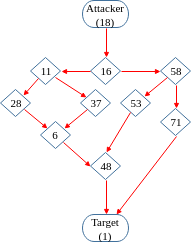
\includegraphics[width=\linewidth,height=6cm]{content/figs/net_ags_003.png}
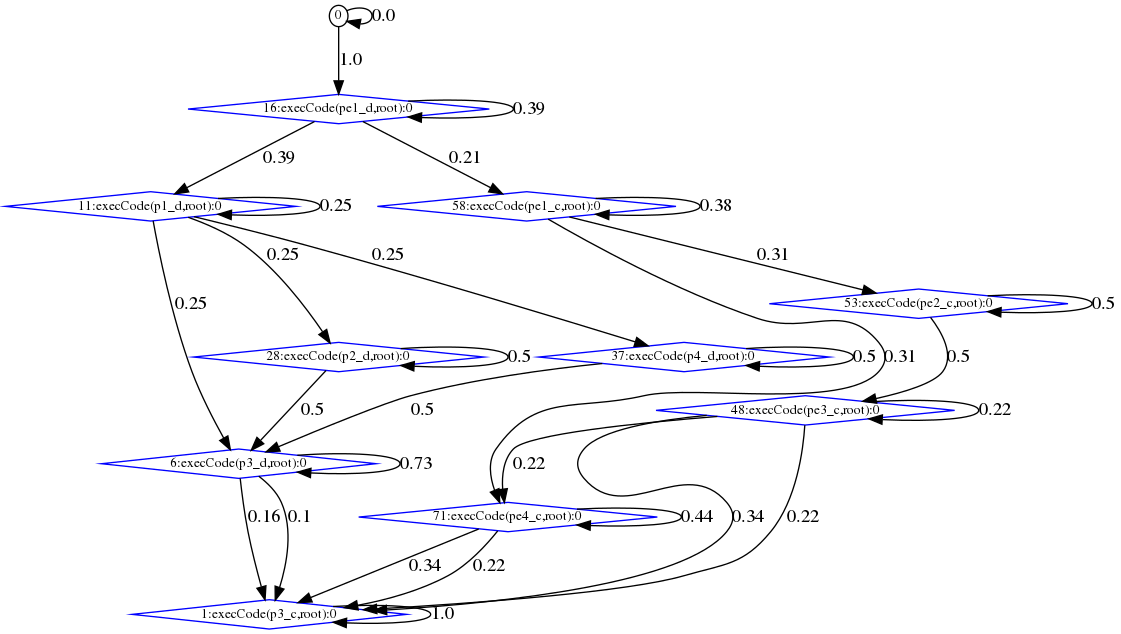
\includegraphics[width=\linewidth,height=6cm]{content/figs/weightedGraphs/current_007_weighEdges.png}
\caption{current}
\label{fig:ag_currt}
\end{subfigure}%
\begin{subfigure}{.33\textwidth}
%%\includegraphics[width=\linewidth,height=6cm]{img/1553187466087.png}
% 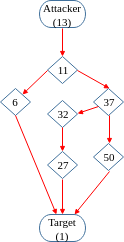
\includegraphics[width=\linewidth,height=6cm]{content/figs/net_ags_002.png}
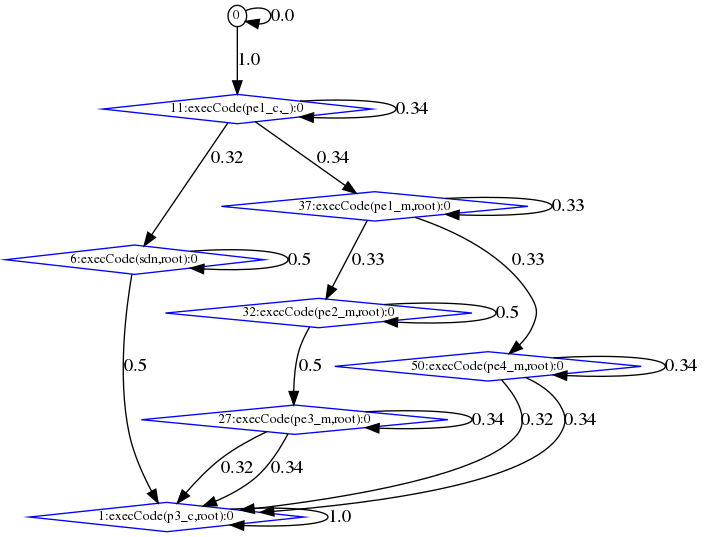
\includegraphics[width=\linewidth,height=6cm]{content/figs/weightedGraphs/transition_007_weighEdges.png}
\caption{transition}
\label{fig:ag_trans}
\end{subfigure}%
\begin{subfigure}{.2\textwidth}
%\includegraphics[width=\linewidth,height=6cm]{img/1553187466083.png}
% 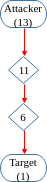
\includegraphics[width=\linewidth,height=5cm]{content/figs/net_ags_001.png}
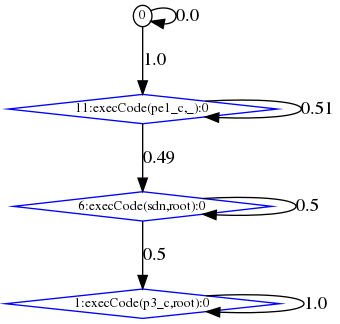
\includegraphics[width=\linewidth,height=5cm]{content/figs/weightedGraphs/final_007_weighEdges.png}
\caption{final}
\label{fig:ag_fut}
\end{subfigure}%
\caption{Generated Attack Graphs}
\label{fig:ag_all}
\end{adjustbox}
\end{figure*} 


\begin{figure*}[ht]
\centering
\begin{adjustbox}{minipage=\linewidth,scale=1}
\begin{subfigure}{.33\textwidth}
\includegraphics[width=\linewidth]{img/1553187466081.png}
\caption{current}
\label{fig:nra_curr}
\end{subfigure}%
\begin{subfigure}{.33\textwidth}
\includegraphics[width=\linewidth]{img/1553187466082.png}
\caption{transition}
\label{fig:nra_trans}
\end{subfigure}%
\begin{subfigure}{.33\textwidth}
\includegraphics[width=\linewidth]{img/epl_final.png}
\caption{final}
\label{fig:nra_fin}
\end{subfigure}%
\caption{Node Rank Analysis}
\label{fig:nr_all}
\end{adjustbox}
\end{figure*} 
